\chapter{Introduction}
\section{Research Question}
\section{Overview}

In the following the structure of the thesis is outlined. Every chapter is briefly discussed, what it is about.

In the second chapter we will walk through the foundations. The chapter mentions technologies, which are used for the thesis and gives references. Furthermore it gives references to the practices which are used and are crucial for the thesis. The references are properly selected, to understand the details if they are not known and to understand what the technologies and techniques are used for. In summary those are kubernetes, continuous delivery, continuous deployment and techniques from infrastructure as code and site reliability engineering.

The third chapter is conceptual macro view to the technique nonfunction production regression testing. The text walks through the general environment and discusses the most important concepts and how they communicate with each other. The most important steps of the continous delivery pipeline are discussed and it explains how the pipeline is extended in order to have the technique of nonfunctional production regression testing. The text argues how the methodologies of nonfunctional production are embedded in the pipeline and how the pipeline must be extended.

In the fourth chapter we will get to the concrete implementation of the nonfunctional production regression testing. The chapter will go into the details of how the concept is implemented. Concretely the software deployer is described, which was implemented in the context of this thesis.

Chapter five is about the evaluation of the new approach. We will investigate the use of the technique and customized software in two different companies. The first company is Gapfish, a four year old startup, and the software department of DIN, a company which is established for a hundred years. We are going to evaluate positive outcomes, still problematic concerns and their improvements. Another part of the evaluation is the comparison to other techniques which other companies and groups developed and tested. We differentiate in their features, advantages and disadvantages.

In the last chapter, the conclusion, the whole thesis is summarized and all the chapters are resumed. Important is the second part of the conclusion, in which we have an outlook to further improvements and how the technique can be extended to have further upgrades to delivery pipelines.

\chapter{Foundations}

\chapter{General Approach}

Nonfunctional Production Regression Testing is the topic of the masterthesis and we will discuss the core of it in this chapter. The designation itself describes precisely what the technique and what the new practice is about. Therefore we will go shorty through every single term in the following.

Nonfunctional refers to the metrics, which we're evaluating in the test; These metrics are only nonfunctional and as a consequence generically applicable to multiple applications. The term production refers to the environment. The metrics, which are collected are collected in the production environment. And finally the term regression refering to the testing strategy. The metrics will be compared between two different versions and the latter version is tested for a regression, concretely a decline of the monitored metrics.

The testing technique provides some further features, which are not included in the designation. Indeed the testing technique is completely automatable and you can continuously apply it to the new versions. The testing technique is designed in respect to failing as fast as possible and inform developers.

When it comes to automation and continuous, the thoughtful reader is now probably reminded of continuous integration, delivery and deployment. This testing techniques evolved naturally from those practices and extends those. Those already established practices support the developers until the software is deployed. In contrast to that, nonfunctional production regression testing, supports the developers during after the deploy and while the software runs in production.

To understand the testing procedure in a whole and completely, it is necessary to show a complete overview of the whole testing and production environment. We will go through the steps of the pipeline and discuss it in a nutshell as you can see in the figures.

\begin{figure}[htbp]
	\centering
	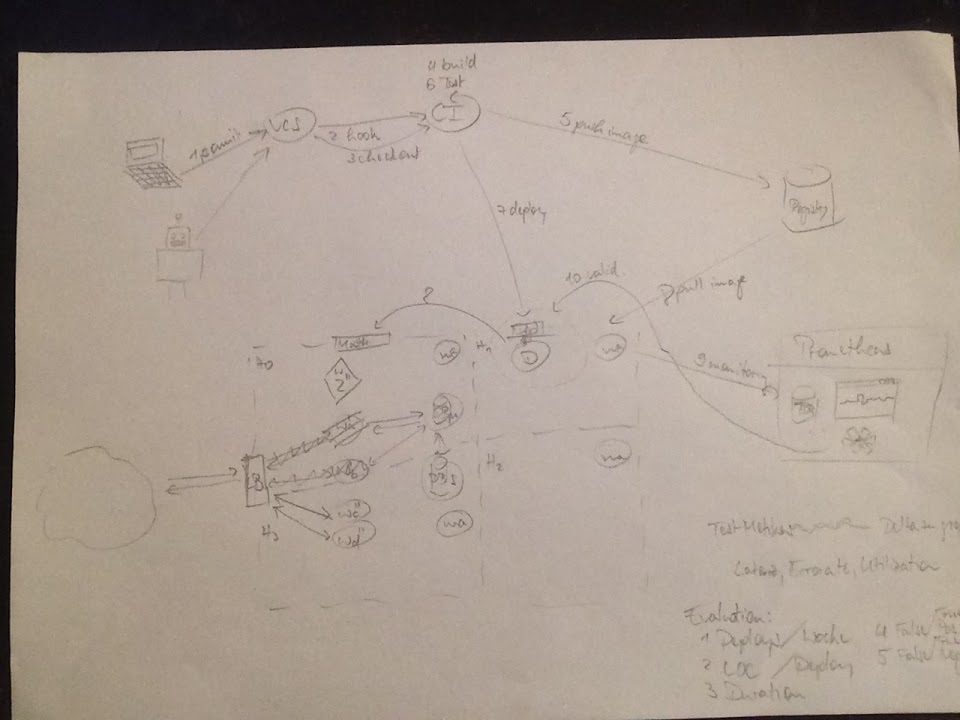
\includegraphics[width=.8 \textwidth]{nprt}
	\caption[GMF Dashboard View]{Nonfunction Production Regression Testing Overview.}
	\label{fig:nprt}
\end{figure}

The steps in the very beginning are known from the established practices continuous delivery and deployment respectively. But it is necessary to touch them and integrate them to the whole picture and outline the special characteristics for the new testing technique.

At the very beginning, there is a developer, who changed the code locally on his working machine. There is also a version control system. And in the first step the developer commits the code to the version control system. The main focus is on git. Subversion is possible, too though. In the following description we will stick to the terms and notions of git.

Next there is a continuous integration system. After the commit happened, the second step is a message to the continuous integration system. The message holds the information that a new commit exists and the continuous integration server clones the code from the version control system and checks out the specified version. Now the continuous integration system has three major jobs. The first one is to start a build process, the second is to run the tests and the third is to give the deploy signal.

In step four, namely running the build, it is typical to compile binaries, render assets and further artifacts. For our purposes it is especially necessary to build at least one or multiple docker images.

The import thing about this is, that we need to identify every docker image to a specific build. Therefore we use the commit hash, the version created by the version control system. This commit hash will follow us through the whole pipeline. This is important to be able to trace every step in the pipeline for a specific version. With this thought in mind, the docker image is tagged with the commit hash of this version and the name of the branch. Along the way it is mentioned, that the branch name is not absolutely necessary to definitely determine the version. The branch name is included for better readability for a developer and approximately recognize what the image version is about.

The continuous integration server then pushes the ready build docker image to an image registry, such as docker hub. Nevertheless this can be a private registry as well. This registry serves later as an artifact repository.

The second continuous integration step, or in total step six, the continuous integration server runs the tests. There can be multiple stages, such as unit, feature or smoke tests. Yet we do net need to recall all the details here.

The last step of the continuous integration system is to send a deploy signal. In the shown figure this is step seven. When you look at the tests, the result could on the one hand be a failure or on the other hand be successful. If the test have failed, the remaining pipeline will be cancelled and the developer will be informed. Just as you know it from a typical continuous integration system. If the tests have been successful and accordingly the build including all test stages have been successful, the continuous integration system sends the signal to deploy.

It makes sense to deploy only specific versions and not every commit. The practice which is pretty common, is that you develop new features in a seperate branch. For those version it is common to not send a deploy signal even though the branch build and tests are successful. Usually after there has been a review and a decision to deploy the changes to production, even though it is a very small change. But when the decision is made and merged into a specified branch, for instance the master branch, this version will go to production.

However, just to clarify, each built image for every single version is sent, independently of successful tests and independently of the intention to go to production, to the image repository. The reason could be a staging system and even running the tests inside the build image. But this is just a side note.

So the deploy signal is given when two requirements are fulfilled: the build and tests are successful and it is a version which is planned to go to production.

Until this point, as it was already mentioned, it is just a usual continuous delivery or deployment pipeline, which is commonly used in the development process. But since nonfunctional production regression testing is a technique, which is supposed to be completely automated, such a prior described delivery pipeline including automated deployments is precondition. From now on it is becoming interesting, hence the testing technique supports the developers post deployment in production instead of the old practices before the deploy.

The next unit is the deployer. It is the software, which is particularly implemented for this masterthesis. In the next chapter the deployer is described in detail. This chapter demonstrates how the deployer is embedded in the pipeline or in other words in the environment amongst all other tools. In the meantime tools exist, which have a similar purpose. It is crucial to have full control over the whole deployment process and as a consequence it was necessary to implement the software and have it customizable.


\chapter{Implementation of the Approach}

\chapter{Evaluation}
\section{Adoption of the approach}
\section{Comparison of to other approaches}

\chapter{Conclusion}
\section{Resume}
\section{Outlook and future work}

% \part{Foundations}

% \chapter{Introduction: Developer and operation teams converge and both use software engineering practices}

% \chapter{Developers use the Continuous Delivery Pipeline}

% \section{The Continuous Delivery Pipeline consists of commitment, continuous integration and deployment}
% \section{Software Deployment approaches evolved from manual to automated}
% \subsection{Blue-Green Deployment allows Zero Downtime releases}

% The approach of blue green deployment involves two environments. One is the environment which serves production traffic, the other environment is in standby. You deploy to the other environment the new version. You then switch routing from the environment, which runs the old version, to the environment with the new version.

% This has the major disadvantage that it is a waste of resources. Just one environment doing work with serving production traffic as the other environment is just idling. Even if you use the idling environment as a staging it would be oversized and still wasting resources.

% \subsection{Automation leads to resource saving Phoenix Deployment and Rolling Deployments}

% In times of dynamic resource allocation, automation and virtual machines, it became easy to automatically spawn new servers. In for a deploy of a new version you would not change the servers, but automatically create new ones with the version to deploy, then switch the traffic from the old servers to the new servers, and in the end just destroy the old servers. This procedure is called phoenix replacement.

% \subsection{Canaries test releases with a small amount of traffic}


% Canary releasing is a way to test new versions of the application in production. But testing in production is risky, because when there is an error which leads to a defect or failure the users will get affected. And this costs money in any way.

% There comes canary releasing into play. A single canary can't do much harm and it's not a big catastrophe if the small canary is malicious. Let me explain it at the example of a typically scaled web application. Usually you do not have just a single web server, but multiple servers. So when releasing in the canary style, you change just a small proportion of the twenty webservers to the new version. Now two versions of the webservers are running at the same time.

% Usually you want exactly the same version of webservers in production with the exact same configuration. This makes systems easier to debug in case of an error. The maximum count of different versions during canary releasing is two. But why go for two different versions in production with the canary releasing technique, when it makes debugging in general harder.

% It's because with canary releasing you can achieve different goals. The first one is truly when an error occurs. Just because less users are affected by the error. The majority of webservers is still in the old version, so just a small portion of all the users have a poor experience with the erroneous small canary version fraction.

% In case of success, when everything works as expected, it is proven that there is less risk of errors, even under real production conditions.


% \subsection{continuous deployment is not continuous delivery}

% \chapter{Operators turned into Site Reliability Engineers}

% Companies, which run software on their servers, usually have a specialized operations team. A team of developers programs the software and after the team is finished, the software is handed to another team, which runs the software and keeps it running. Those teams are usually referred as operations teams. So what are their duties and responsibilities exactly?

% At first the already developed software needs to be deployed on an infrastructure. Therefore the operations team must provide an infrastructure. Infrastructure generally consists of hardware like racks, servers and networking devices. But in most cases, software depends on other software components and services, which are for example programming languages, dns or databases. Software usually changes. Most importantly there are security patches, but also software updates with new features are mandatory to install. Hence the operations team is responsible for installing, configuring and updating hardware and software components.

% To provide a certain quality of service, infrastructure as well as the software must be maintained. That means identifying any problems and moreover fixing the identified problems. To identify problems in the first place, there must be any kind of monitoring. A good monitoring system\cite[p. 127/8]{devops} finds failures and resulting faults, recognizes performance problems, usual workloads and it detects intruders. More obvious problems can be detected early, even before the problem leads to failures. For example a disk will soon be full or utilization of resources like cpu, ram, network or disk i/o is too high. Other failures can not be detected in advance and lead to a defective system.

% In case monitoring identifies a problem, the operations team needs to take care of the problem. Operations teams need to be on call and manage incidents. A new Incident must be rated how severe it is. In advance detected problems potentially leading to failures like a disk going to be full in few days, must not be handled immediately. Other incidents like an unavailable database service can be business critical and must be fixed as rapidly as possible. But often the cause of a failure is not obvious and the system must be debugged with specific tools. Critical failures mostly affect users, so another part of incident management is to inform the affected parties.

% Google states that the traditional approach of an operations team\footnote{Google actually calls it the sysadmins approach} is not efficient. It is expensive, it does not scale very well and it creates tension in interests\cite[p. 3/4]{site_reliability}.

% A growing system means there will be more hardware, more software components and a more complex configuration. More people are needed to install, monitor and maintain the infrastructure and services. The traditional operations team approach has the disadvantage, that it does not scale very well and produces more costs, the bigger the system becomes. Another disadvantage is conflicting interests of the developer team and operation team. Operations teams are payed to create stability and provide a certain quality of service. But change is the biggest source of failure\cite[p.10]{site_reliability}. That's why operations teams work under the motto of 'Never change a running system'. On the other hand, a good service changes to the needs of its users. Developers get paid to deliver as much features as possible, so they want frequent change. Those are conflicting interests and they harm the whole product. For Google it's clear, that the different assumptions and tension in interests of operations and developer teams produce a lot of hidden costs.

% \section{Site Reliability Engineers maintain systems like software engineers}

% Operations teams developed a lot of practices to both integrate the fundamentally conflicting interests of change and stability, but also scale the operations team approach. This reduces obvious and hidden costs and makes the whole work more efficient. A lot of those practices became possible, because the infrastructure turned from pure hardware into a dynamic software defined infrastructure. Google refers to this approach as the site reliability engineering approach. It is operations how an software engineer would do it.

% New technologies made it possible to define all infrastructure in code. One of the first who provided an dynamic infrastructure is amazon with ec2. The technology of virtualization made provisioning and configuration to software tasks instead of hardware tasks. This is what it made automate-able. Also Docker made it easier to package software and to deploy and configure the services\footnote{See Chapter 2 'Platforms' in \cite{infra_as_code} for those technologies}.

% With the possibility to automate the tasks an operations team has to do, there will come many benefits. The obvious value is that is scalabillity. When a task is automated and can be done by a machine, it is very cheap and easy to execute the task a lot more often. But there is a much bigger advance, which automation gives. When a task is automated it is a well defined process, which will consistently performed, where a human can easily make a mistake by manually executing the task. It can also be extended, measured and done at inconvenient times for humans\footnote{See Chapter 'Value of Automation' in \cite{site_reliability} for complete discussion of the advantages.}.

% The before one off tasks of provisioning, deploying and configuring have now well defined practices and processes. Those tasks are now reproducible because the definition or configuration of the infrastructure can now be stored in a version control system. And with automate-able deployment processes like zero downtime releases, phoenix deployment or rolling updates, those processes can be done continuously.

% Operations teams have collected great knowledge on monitoring. What are the key indicators for monitoring a system. What does a good monitoring infrastructure provide. Those questions I am going to examine in detail in the upcoming sections. But very important is that monitoring can notify a human or even better trigger automated tasks, that humans do not need to be involved at all, when a problem occurs.

% Also incident management can partly be automated. Distributed systems like databases have nowadays automatic failovers. Issues which have been serious, major incidents before and a humans had to manually intervene can, are now automatically triggered and the systems heal themselves. Disaster recovery is now easily done, because you can automatically reprovision the whole infrastructure as mentioned before.

% With those practices it means that in the end this means that the conflicting interests of change and stability can nowadays be more and more integrated.

% \section{Monitoring to identify Problems}
% \subsection{Health checks measure availability}
% \subsection{Measuring Latency, Traffic, Errors and Saturation identifies failures and performance problems}
% \subsection{Incident Management (/Notifications) for appropriate and fast actions in case of Problems}

% \chapter{Metrics measure team efficiency and software quality}
% \section{Velocity and cycletime are efficiency metrics for an agile team}
% cycle time measures quality of delivery engine
% \subsection{Deploys/Week indirectly measures velocity}
% and it measures the effect of a quality delivery engine
% we want many deploys per week
% \subsection{Deploy Duration is import for cycle time}
% \section{MTTR and Failurerate measure the quality of a software}
% we want low risk per deploy to achieve MTTR and low Failure Rate
% \subsection{LOCS/Deploy indirectly measures the risk per deploy}


% \part{New Practices}

% \chapter{Post Release Testing extends the Continuous Delivery Pipeline to support maintaining a system}

% The three main steps in the continuous delivery pipeline are: commitment to version control, continuous integration and release. After releasing, the new version will be operated. This includes monitoring, logging, security aspects and incident management\footnote{In ``Site Reliability Engineering'' monitoring and notifying principles~\cite[p. 55-63]{site_reliability} are well described.}. To enable developers to take more responsible in running the software, it is necessary to extend the practices of the continuous delivery pipeline.

% In my masterthesis I want to optimize the software engineering practices in order to empower developers in their bigger responsibilities. I want to focus on the process of deployment and enhance the continuous delivery pipeline. To achieve this, I want to examine operation practices like monitoring and incident management. And then extend the deployment process by three consecutive steps.

% The first step is to completely automate deployments of software features and achieve continuous deployment. The next step is to sensibly monitor new releases to give automatically feedback. Third and lastly, identify incidents to automatically trigger rollbacks to self-heal the software system. I'm going to call these last two steps continuous post release testing.

% \section{Post Release Testing leads to lower time to market}
% cycle time
% \section{It makes Releases consistent, measurable, fast and scalable}
% mttr, automation/automatic discussion
% \section{It is a new opportunity for risk management}
% identify test before release is a mttr of zero, after release still fast. easier to test in production (complexity of system)
% \section{Companies are already post release testing their software systems}
% \subsection{Netflix uses Simian Army to live test their systems}
% \subsection{Synthetic Monitoring tests a complex distributed system}
% \section{Post Release Testing with Canaries is appropriate for testing non change}
% ErrorRate as monitoring measure for automation
% problems in error rate measure defect and failure
% solution a secific heuristic
% \subsection{Black-Box monitoring is only one part and monitoring change is difficult}
% \subsection{Canary testing is important for maintenance but not feature deploys}
% \subsection{Continuous Delivery is a requirement}
% \subsection{Notifications in case a canary behaves different}
% \subsection{Automated Rollbacks for a automatic self healing system}

% \chapter{Implementing Canary Post Release Testing}
% \section{New technologies drive new techniques}
% \subsection{Kubernetes is a Cluster OS}
% \subsubsection{Resource Management in Kubernetes is made for high available services}
% \subsubsection{Deployments implement Rolling Updates}

% The extend to the canary releasing technique is a rolling update. It unifies phoenix replacement and canary releasing and extends it to a full deployment. You start with one server in the new version and spawn it automatically. Now it becomes part of the whole pool of servers and serves traffic as the server is ready. Now two different versions are serving traffic, just like with a canary release. But after the first step the deployment goes on and then destroys a server instance in the old version as you would do in the phoenix replacement. Then the procedure will be done multiple times until all servers of the old version are replaced by the new version.

% \subsection{DataDog is a Cluster Monitoring Systems as a sevice}
% alternativen Graphana, Prometheus
% \subsubsection{The main components are: Datacollection, Timeseriesdatabase, Graphing and Alerting}
% \subsubsection{DataDog integrates well in Kubernetes}
% \section{Deployer is a Service for Continuous Deployment and enables Canary Post Release testing}
% \subsection{Deployer integrates into the Continuous Delivery Pipeline}
% \subsection{Deployer integrates into Kubernetes and deploys itself}
% \subsection{Deployer integrates into Monitoring and enables Canary testing}
% \subsection{The main Deployer API features are Deployments and Canary deployments}
% depctl, curl
% \subsubsection{Deployments deploy a whole repository}
% \subsubsection{One Canary per Replicated Pods can be deployed and monitored}
% \subsubsection{Immediate Notifications in case of failure}
% difference depctl and curl
% \subsubsection{Automatic Rollbacks in case defect Canary}
% via datadog and triggers deployer
% future: staging deploys

% % \subsection{bugs + debugging}
% % \subsection{ilities}
% % \subsection{security}
% % \subsection{monitoring}


% \part{Evaluation}

% \chapter{GapFish is the company to evaluate Deployer}
% \section{GapFish's services are complex and highly available}
% overview of Gapfish's services
% \subsection{GapFish's Operation Service is used by internal Staff and Customers}
% operation service == operation.gapfish.com
% \section{GapFish uses tools for continuous deployment}
% \subsection{GapFish differentiates between development and operation}
% how is the deployment tradditionally done
% \subsection{Kubernetes enables GapFish to have development and operations in one team}
% which services are migrated to kubernetes

% \chapter{Metrics are implemented as logging output}
% \section{Deploys/Week}
% \section{Deploy Duration}
% \section{LOCS/Deploy}

% \chapter{Results}
% \section{Metrics: traditional vs. new approach}
% \section{theoretical/practical conclusion for deployer and cd}
% \section{for Gapfish}
% \section{Lessons learned and future}

% \chapter{resume}
